\documentclass[border=15pt]{standalone}
\usepackage{amsmath, amssymb}
\usepackage{tikz}
\usetikzlibrary{arrows.meta}

\definecolor{block0}{HTML}{E53935}
\definecolor{block1}{HTML}{1E88E5}

\begin{document}
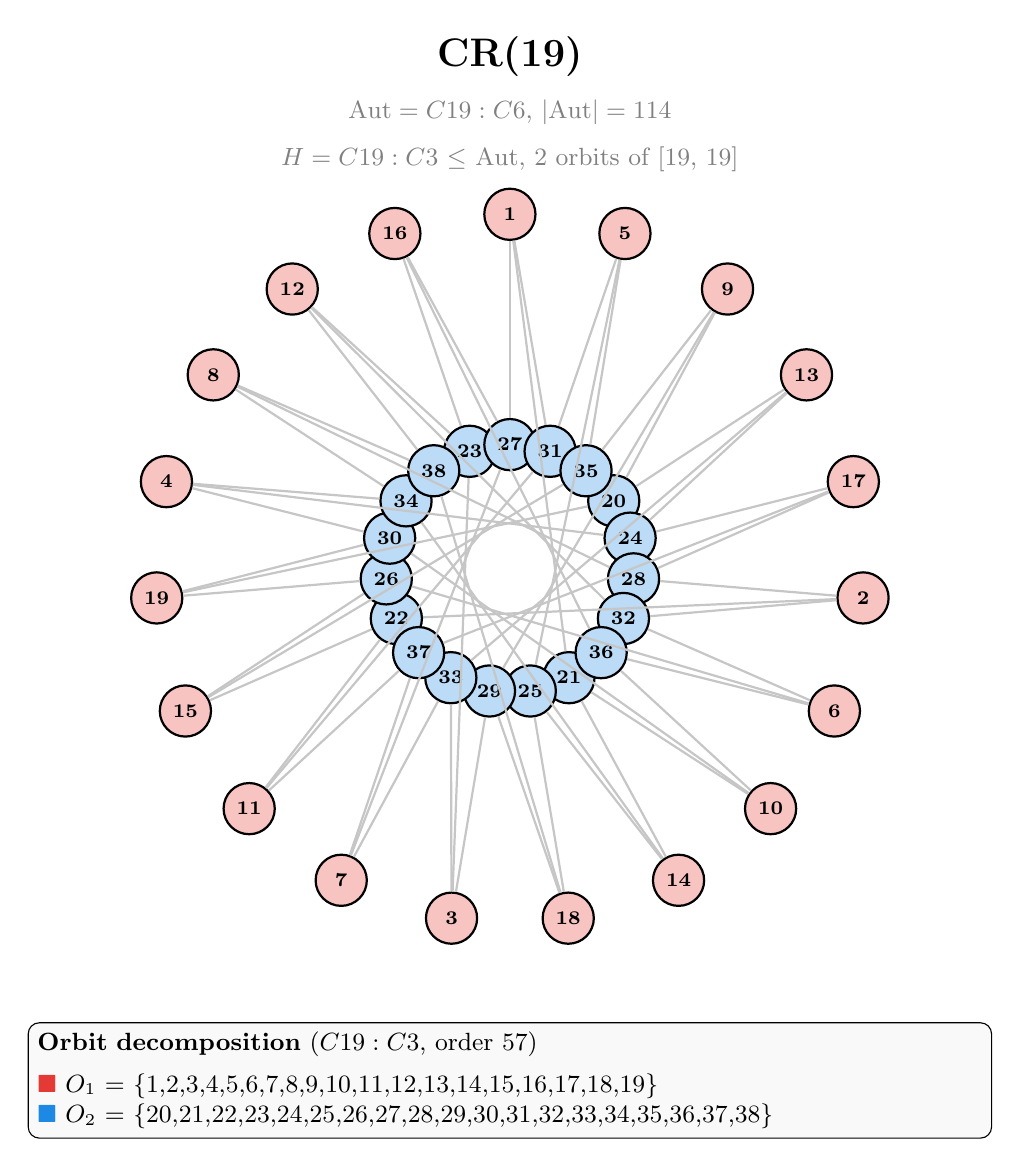
\begin{tikzpicture}[
  vertex/.style={circle, draw, thick, minimum size=6.5mm, inner sep=0pt,
                 font=\scriptsize\bfseries},
  edge/.style={thick, gray!45},
  title/.style={font=\Large\bfseries},
  subtitle/.style={font=\small, text=gray},
]

\node[title] at (0, 6.5) {CR(19)};
\node[subtitle] at (0, 5.8) {$\mathrm{Aut} = C19 : C6$, $|\mathrm{Aut}| = 114$};
\node[subtitle] at (0, 5.2) {$H = C19 : C3$ $\leq$ $\mathrm{Aut}$, 2 orbits of [19, 19]};

\node[vertex, fill=block0!30] (v1) at (0.000, 4.500) {1};
\node[vertex, fill=block0!30] (v2) at (4.485, -0.372) {2};
\node[vertex, fill=block0!30] (v3) at (-0.741, -4.439) {3};
\node[vertex, fill=block0!30] (v4) at (-4.362, 1.105) {4};
\node[vertex, fill=block0!30] (v5) at (1.461, 4.256) {5};
\node[vertex, fill=block0!30] (v6) at (4.121, -1.808) {6};
\node[vertex, fill=block0!30] (v7) at (-2.142, -3.958) {7};
\node[vertex, fill=block0!30] (v8) at (-3.767, 2.461) {8};
\node[vertex, fill=block0!30] (v9) at (2.764, 3.551) {9};
\node[vertex, fill=block0!30] (v10) at (3.311, -3.048) {10};
\node[vertex, fill=block0!30] (v11) at (-3.311, -3.048) {11};
\node[vertex, fill=block0!30] (v12) at (-2.764, 3.551) {12};
\node[vertex, fill=block0!30] (v13) at (3.767, 2.461) {13};
\node[vertex, fill=block0!30] (v14) at (2.142, -3.958) {14};
\node[vertex, fill=block0!30] (v15) at (-4.121, -1.808) {15};
\node[vertex, fill=block0!30] (v16) at (-1.461, 4.256) {16};
\node[vertex, fill=block0!30] (v17) at (4.362, 1.105) {17};
\node[vertex, fill=block0!30] (v18) at (0.741, -4.439) {18};
\node[vertex, fill=block0!30] (v19) at (-4.485, -0.372) {19};
\node[vertex, fill=block1!30] (v20) at (1.319, 0.861) {20};
\node[vertex, fill=block1!30] (v21) at (0.750, -1.385) {21};
\node[vertex, fill=block1!30] (v22) at (-1.442, -0.633) {22};
\node[vertex, fill=block1!30] (v23) at (-0.511, 1.490) {23};
\node[vertex, fill=block1!30] (v24) at (1.527, 0.387) {24};
\node[vertex, fill=block1!30] (v25) at (0.259, -1.554) {25};
\node[vertex, fill=block1!30] (v26) at (-1.570, -0.130) {26};
\node[vertex, fill=block1!30] (v27) at (0.000, 1.575) {27};
\node[vertex, fill=block1!30] (v28) at (1.570, -0.130) {28};
\node[vertex, fill=block1!30] (v29) at (-0.259, -1.554) {29};
\node[vertex, fill=block1!30] (v30) at (-1.527, 0.387) {30};
\node[vertex, fill=block1!30] (v31) at (0.511, 1.490) {31};
\node[vertex, fill=block1!30] (v32) at (1.442, -0.633) {32};
\node[vertex, fill=block1!30] (v33) at (-0.750, -1.385) {33};
\node[vertex, fill=block1!30] (v34) at (-1.319, 0.861) {34};
\node[vertex, fill=block1!30] (v35) at (0.967, 1.243) {35};
\node[vertex, fill=block1!30] (v36) at (1.159, -1.067) {36};
\node[vertex, fill=block1!30] (v37) at (-1.159, -1.067) {37};
\node[vertex, fill=block1!30] (v38) at (-0.967, 1.243) {38};

\draw[edge] (v1) -- (v21);
\draw[edge] (v1) -- (v27);
\draw[edge] (v1) -- (v31);
\draw[edge] (v2) -- (v22);
\draw[edge] (v2) -- (v28);
\draw[edge] (v2) -- (v32);
\draw[edge] (v3) -- (v23);
\draw[edge] (v3) -- (v29);
\draw[edge] (v3) -- (v33);
\draw[edge] (v4) -- (v24);
\draw[edge] (v4) -- (v30);
\draw[edge] (v4) -- (v34);
\draw[edge] (v5) -- (v25);
\draw[edge] (v5) -- (v31);
\draw[edge] (v5) -- (v35);
\draw[edge] (v6) -- (v26);
\draw[edge] (v6) -- (v32);
\draw[edge] (v6) -- (v36);
\draw[edge] (v7) -- (v27);
\draw[edge] (v7) -- (v33);
\draw[edge] (v7) -- (v37);
\draw[edge] (v8) -- (v28);
\draw[edge] (v8) -- (v34);
\draw[edge] (v8) -- (v38);
\draw[edge] (v9) -- (v20);
\draw[edge] (v9) -- (v29);
\draw[edge] (v9) -- (v35);
\draw[edge] (v10) -- (v21);
\draw[edge] (v10) -- (v30);
\draw[edge] (v10) -- (v36);
\draw[edge] (v11) -- (v22);
\draw[edge] (v11) -- (v31);
\draw[edge] (v11) -- (v37);
\draw[edge] (v12) -- (v23);
\draw[edge] (v12) -- (v32);
\draw[edge] (v12) -- (v38);
\draw[edge] (v13) -- (v20);
\draw[edge] (v13) -- (v24);
\draw[edge] (v13) -- (v33);
\draw[edge] (v14) -- (v21);
\draw[edge] (v14) -- (v25);
\draw[edge] (v14) -- (v34);
\draw[edge] (v15) -- (v22);
\draw[edge] (v15) -- (v26);
\draw[edge] (v15) -- (v35);
\draw[edge] (v16) -- (v23);
\draw[edge] (v16) -- (v27);
\draw[edge] (v16) -- (v36);
\draw[edge] (v17) -- (v24);
\draw[edge] (v17) -- (v28);
\draw[edge] (v17) -- (v37);
\draw[edge] (v18) -- (v25);
\draw[edge] (v18) -- (v29);
\draw[edge] (v18) -- (v38);
\draw[edge] (v19) -- (v20);
\draw[edge] (v19) -- (v26);
\draw[edge] (v19) -- (v30);

\node[draw, rounded corners, fill=gray!5, text width=12cm, align=left, font=\small]
  at (0, -6.5) {
  \textbf{Orbit decomposition} ($C19 : C3$, order 57) \\[4pt]
  \textcolor{block0}{$\blacksquare$} $O_{1}$ = \{1,2,3,4,5,6,7,8,9,10,11,12,13,14,15,16,17,18,19\} \\
  \textcolor{block1}{$\blacksquare$} $O_{2}$ = \{20,21,22,23,24,25,26,27,28,29,30,31,32,33,34,35,36,37,38\}
};

\end{tikzpicture}
\end{document}